\chapter{有限元无网格混合离散方案}

第二章介绍的混合离散方案压力节点要依附单元上,无法任意布置。为了使压力自由度达到最优,在所提出的混合公式中,使用传统有限元法来近似位移,采用再生核无网格法来近似压力。
\section{再生核近似}
如图\ref{ch_4:fig:meshfree}所示,再生核无网格近似将求解域$\Omega$及其边界$\Gamma$由$n_p$个无网格节点离散$\{\boldsymbol x_I\}_{I=1}^{n_p}$。每个无网格节点$\boldsymbol x_I$对应的形函数为$\Psi_I(\boldsymbol{x})$,形函数影响域为$supp(\boldsymbol{x}_I)$,并要求影响域的覆盖域需包含求解域$\Omega$,即$\Omega\subseteq^{n_p}_{I=1}supp(\boldsymbol{x}_I)$。考虑求解域$\Omega$内的一个变量$u(\boldsymbol{x})$,其对应的无网格近似函数$u_h(\boldsymbol{x})$可表示为:
\begin{equation}
    u_h(\boldsymbol x) = \sum_{I=1}^{n_p} \Psi_I(\boldsymbol x) d_I
\end{equation}
其中$d_I$为与无网格节点$\boldsymbol{x}_I$对应的节点系数。
\begin{figure}[H]
    \centering 
        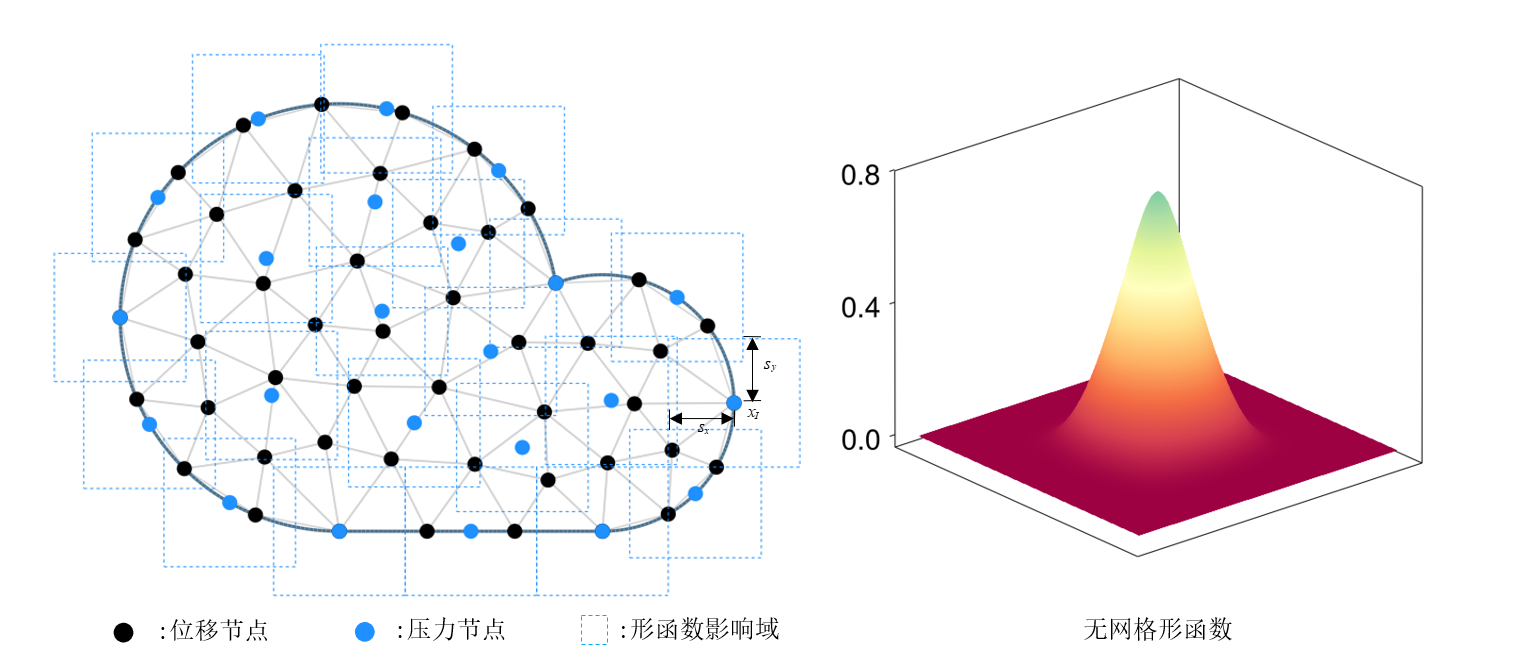
\includegraphics[scale=0.7]{figures/meshfree.png}
        \caption{无网格离散示意图}\label{ch_4:fig:meshfree}
\end{figure}

根据再生核近似理论\cite{liu1995},无网格形函数可以假设为如下形式:
\begin{equation}\label{ch_4:eq:rkshape}
    \Psi_I(\boldsymbol x) = \boldsymbol c(\boldsymbol x_I-\boldsymbol x) \boldsymbol p^{[n]}(\boldsymbol x_I-\boldsymbol x) \phi(\boldsymbol x_I - \boldsymbol x)
\end{equation}
其中$\boldsymbol p$为$n$阶基函数向量,其表达式为:
\begin{equation}
    \boldsymbol p^{[n]}(\boldsymbol x) = \{ 1, x, y, x^2, xy, y^2,...,y^n\}^\mathrm{T}
\end{equation}
而$\phi$为核函数,其影响域的大小由影响域尺寸$s$决定,核函数及其影响域的大小共同决定了无网格形函数的局部紧支性和光滑性。在二维情况下,核函数的影响域通常为圆形或者矩形。本文的影响域形状为矩形,矩形影响域的核函数可由下列公式计算得到:
\begin{equation}
    \phi(\boldsymbol x_I-\boldsymbol x) = \phi(r_x) \phi(r_y), \quad r_x = \frac{|\boldsymbol x_I - \boldsymbol x|}{s_{x}},r_y = \frac{|\boldsymbol y_I - \boldsymbol y|}{s_{y}}
\end{equation}
其中, $s_x$ 和 $s_y$ 分别为 $x$ 和 $y$ 方向上的影响域尺寸,若节点均匀布置,一般使两个方向上的影响域大小相等,即$s_x = s_y = s$。
为保证形函数的紧支性和光滑性,$\phi$ 通常取为阶次大于 $n$ 的紧支函数。对于弹性力学问题,无网格基函数一般选择二阶或者三阶多项式基函数,核函数 $\phi(\boldsymbol x_I-\boldsymbol x)$ 取为三次样条函数:
\begin{equation}
    \phi(s) =\frac{1}{3!} \begin{cases}
        (2-2s)^3 - 4(1-2s)^3 & s\le\frac{1}{2} \\
        (2-2s)^3 &\frac{1}{2}<s<1 \\
        0 & s> 1
    \end{cases}
\end{equation}
$\boldsymbol c$为待定系数向量,可以通过满足下列一致性条件确定:
\begin{equation}\label{ch_4:eq:cc1}
    \sum_{I=1}^{n_p}\Psi_I(\boldsymbol x) \boldsymbol p^{[n]}(\boldsymbol x_I) = \boldsymbol p^{[n]} (\boldsymbol x)
\end{equation}
或等效的转换形式:
\begin{equation}\label{ch_4:eq:cc2}
    \sum_{I=1}^{n_p}\Psi_I(\boldsymbol x) \boldsymbol p^{[n]}(\boldsymbol x_I-\boldsymbol x) = \boldsymbol p^{[n]} (\boldsymbol 0)
\end{equation}
将式\eqref{ch_4:eq:rkshape}代入式\eqref{ch_4:eq:cc2}中即可得到待定系数向量$\boldsymbol c$的具体表达式:
\begin{equation}\label{ch_4:eq:correction}
    \boldsymbol c(\boldsymbol x_I-\boldsymbol x) = \boldsymbol A^{-1}(\boldsymbol x_I-\boldsymbol x)\boldsymbol p^{[n]}(\boldsymbol 0)
\end{equation}
式中$\boldsymbol A$为矩量矩阵:
\begin{equation}
    \boldsymbol A(\boldsymbol x_I-\boldsymbol x) = \sum_{I=1}^{n_p}\boldsymbol p^{[n]}(\boldsymbol x_I-\boldsymbol x) \boldsymbol p^{[n]\mathrm{T}}(\boldsymbol x_I-\boldsymbol x)\phi(\boldsymbol x_I-\boldsymbol x)
\end{equation}

将式\eqref{ch_4:eq:correction}代入式\eqref{ch_4:eq:rkshape}可得最终的再生核无网格形函数表达式:
\begin{equation}\label{ch_4:eq:mfshapefunction}
    \Psi_I(\boldsymbol x) = \boldsymbol p^{[n]\mathrm{T}}(\boldsymbol 0) \boldsymbol A^{-1}(\boldsymbol x_I-\boldsymbol x)p^{[n]}(\boldsymbol x_I-\boldsymbol x)\phi(\boldsymbol x_I-\boldsymbol x)
\end{equation}

\section{有限元无网格混合离散}
从图\ref{ch_4:fig:meshfree}中可以看出,无网格形函数全域高阶连续光滑使得伽辽金无网格法可以不受单元的限制布置节点,能在保证计算精度的情况下,调整体积约束比,达到最优体积约束比。

采用有限元无网格混合离散方案,伽辽金弱形式\eqref{ch_2:eq:weak_mix}中的位移$\boldsymbol{u}$和压力$p$采用不同的离散方式进行近似。位移$\boldsymbol{u}$仍采用有限元形函数\eqref{ch_2:eq:u_h_mix}进行近似,而压力$p$通过无网格形函数\eqref{ch_4:eq:mfshapefunction}进行近似,近似的压力$p_h$可表示为:
\begin{equation}
    p_h(\boldsymbol x) = \sum_{K=1}^{n_p} \Psi_K(\boldsymbol x) p_K
\end{equation}
其中$p_K$为与无网格节点$x_K$对应的节点系数。

\section{数值算例}
\subsection{悬臂梁问题}

首先考虑经典弹性力学二维悬臂梁问题,如图\ref{ch_4:fig:cantilever}所示,悬臂梁的长和宽分别为$L=48$,$D=12$,同时悬臂梁的左端为固定支座,
右端沿着$y$轴正方向施加外部荷载$P=1000$。悬臂梁的材料系数为杨氏模量$E=3\times10^6$、泊松比$\nu=0.5-10^{-8}$。
\begin{figure}[!h]
    \centering 
        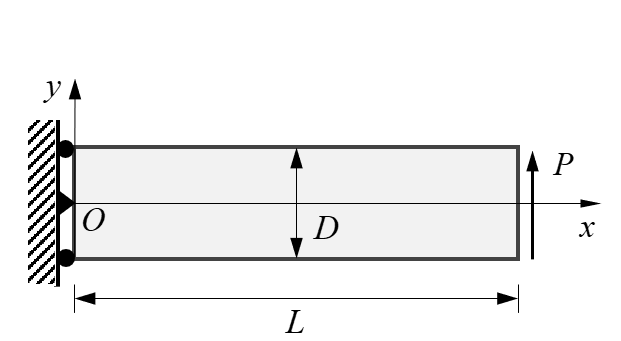
\includegraphics[scale=1.0]{figures/cantilever.png}
        \caption{悬臂梁问题模型}\label{ch_4:fig:cantilever}
\end{figure}

根据圣维南原理和平面应力假设,悬臂梁问题的解析解为:
\begin{equation}
    \begin{split}
        u_1 &= -\frac{Py}{6EI}[(6L-3x)x + (2+\nu)(y^2 - \frac{D^2}{4})] \\
        u_2 &= \frac{P}{6EI}[3\nu y^2(L-x) + (4+5\nu)\frac{D^2x}{4} + (3L-x)x^2]
    \end{split}
\end{equation}
与之相对应的应力分量为:
\begin{equation}
\begin{split}
   \sigma_{xx}&=-\frac{P(L-x)y}{I}\\
   \sigma_{yy}&=0\\
   \sigma_{xy}&=\frac{P}{2I}(\frac{D^2}{4}-y^2)
\end{split}
\end{equation}

\subsection{带孔方板问题}

考虑经典的带孔方板问题,如图\ref{ch_4:fig:hole}所示,板的的中心存在一半径为$a=1$的圆形小孔,同时平板的无穷远处沿$x$轴方向施加均布荷载$T=1000$。 板的材料系数为杨氏模量$E=3\times10^6$、泊松比$\nu=0.49999$。根据Michell解可以得到该带孔无限大平板问题的解析解为:
\begin{equation}
    \begin{split}
        u_x(r,\theta)&=\frac{Ta}{8\mu}(\frac{r}{a}(k+1)\cos\theta-\frac{2a^3}{r^3}\cos3\theta    +\frac{2a}{r}((1+k)\cos\theta+\cos3\theta))\\
        u_y(r,\theta)&=\frac{Ta}{8\mu}(\frac{r}{a}(k-3)\sin\theta-\frac{2a^3}{r^3}\sin3\theta    +\frac{2a}{r}((1-k)\sin\theta+\sin3\theta))  
    \end{split}
\end{equation}
其中,$k$和$\mu$分别为:
\begin{equation}
    \begin{split}
        k=\frac{3-\nu}{1+\nu}\quad \text{,}\mu=\frac{E}{2(1+\nu)}
    \end{split}
\end{equation}
与之相对应的应力分量为:
\begin{equation}
\begin{split}
    \sigma_{xx}&=T(1-\frac{a^2}{r^2}(\frac{3}{2}\cos2\theta+\cos4\theta)+\frac{3a^4}{2r^4}\cos4\theta)\\
    \sigma_{yy}&=-T(\frac{a^2}{r^2}(\frac{1}{2}\cos2\theta-\cos4\theta)+\frac{3a^4}{2r^4}\cos4\theta)\\
    \sigma_{xy}&=-T(\frac{a^2}{r^2}(\frac{1}{2}\sin2\theta+\sin4\theta)-\frac{3a^4}{2r^4}\sin4\theta)\\
\end{split}
\end{equation}

\begin{figure}[!h]
    \centering 
        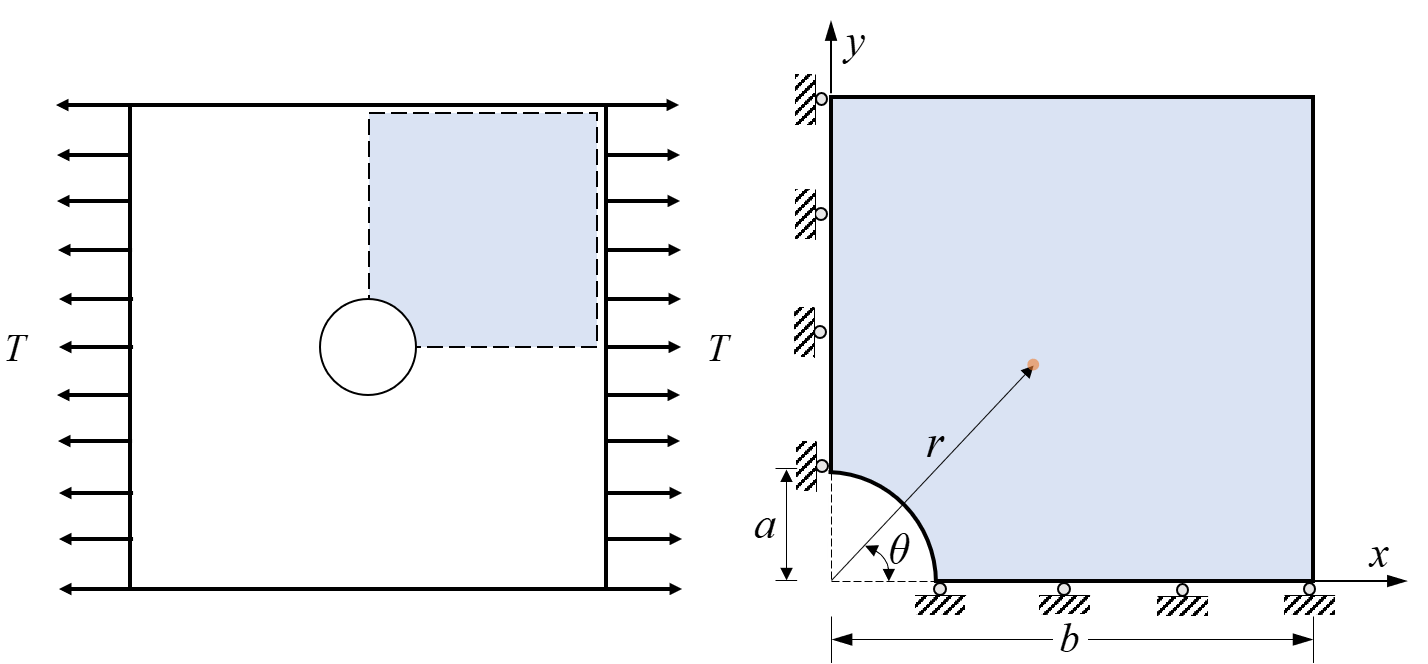
\includegraphics[scale=0.5]{figures/hole.png}
        \caption{带孔方板问题模型}\label{ch_4:fig:hole}
\end{figure}

\subsection{Cook membrane 问题}
考虑经典的Cook membrane 问题,膜的尺寸如图\ref{ch_4:fig:cook}所示,右端沿着$y$轴正方向施加外部荷载$P=6.25$,膜的材料系数为杨氏模量$E=70$、泊松比$\nu=0.5-10^{-8}$。在这种情况下,$A$点的位移参考解为:$u=28$。
\begin{figure}[!h]
    \centering 
        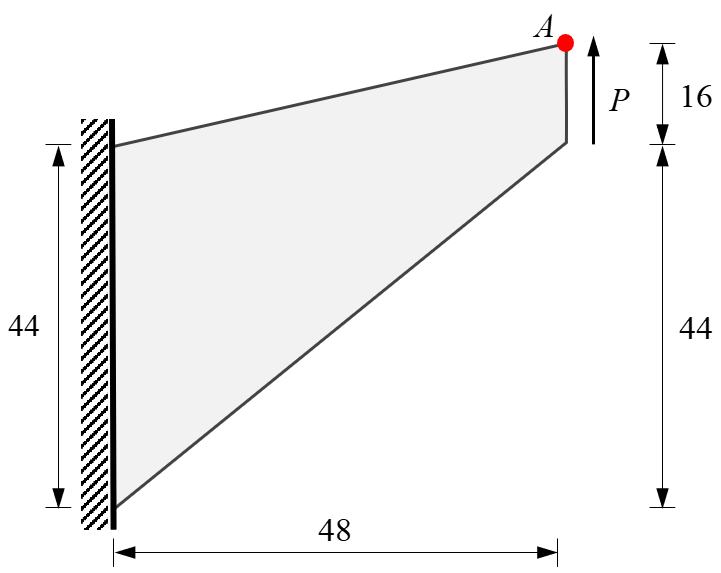
\includegraphics[scale=0.8]{figures/cook.png}
        \caption{Cook membrane 问题模型}\label{ch_4:fig:cook}
\end{figure}

\subsection{方块受压问题}
考虑经典的方块受压问题,方块的尺寸如图\ref{ch_4:fig:cube}所示,方块顶面上施加外部均布荷载$P=80$,方块的材料系数为杨氏模量$E=240.56839$、泊松比$\nu=0.5-10^{-8}$。
\begin{figure}[!h]
    \centering 
        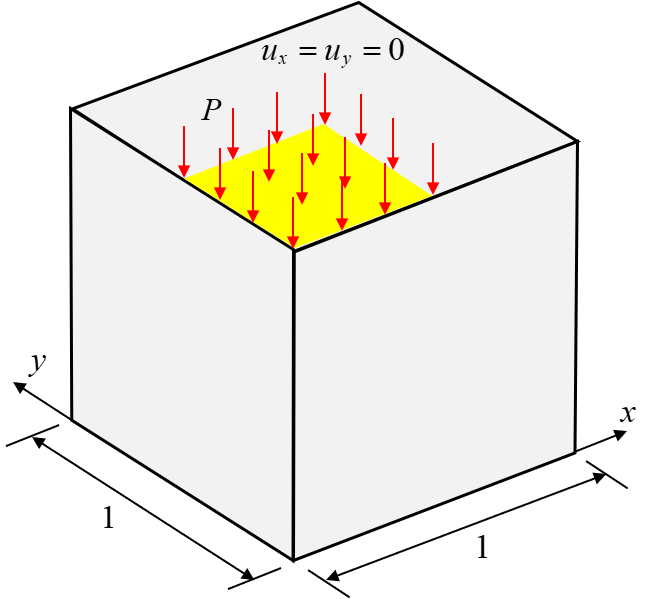
\includegraphics[scale=0.8]{figures/cube.png}
        \caption{方块受压问题模型}\label{ch_4:fig:cube}
\end{figure}

\section{小结}


